\documentclass[a4paper]{article}

\usepackage{amsmath}
\usepackage{url}
\usepackage{acronym}
\usepackage[pdftex]{graphicx}


\acrodef{PDF}[PDF]{Probability Density Function}
\acrodef{GMM}[GMM]{Gaussian Mixture Model}
\acrodef{NB}[NB]{Naive Bayes}
\acrodef{kNN}[kNN]{k-Nearest Neighbour}

\begin{document}

\title{MLPM project \\ The effect of smoothness}
\author{Maarten van der Velden \\ 5743087 \\ \texttt{Maarten.vanderVelden@student.uva.nl} \and Carsten van Weelden \\ 0518824 \\ \texttt{cweelden@science.uva.nl}}
\maketitle

%\begin{abstract}
%\small \textit{ }
%\end{abstract}

\acresetall

\section{Introduction}
\label{sec:introduction}

In this paper we investigate the effect of smoothness of the dataset on the performance of classification algorithms. In order to investigate this we generate several artificial datasets of varying smoothness and look at the accuracy and loss of the resulting classifiers. In order to get insight into the effects we decompose the loss into its bias, variance, and noise components as defined in \cite{Domingos2000}.


To investigate the effect that smoothness has on classification performance we first need to define some idea of smoothness which we can easily vary and then run a set of experiments for different levels of smoothness. We view classification as a two class problem\footnote{As contrasted with a concept learning problem, in which there is one class which needs to be distinguished from the background.}, with each class being represented by some \ac{PDF} over the attribute space. Given this view the \emph{smoothness} of a class is determined by the shape of the \ac{PDF}. We define the \ac{PDF} for each class as a \ac{GMM} with $k$ mixture components. Intuitively, the smoothness is then determined by the number of components in the mixture. With just one component the \ac{PDF} corresponds to a Gaussian distribution which is very smooth, while increasing the number of components increases the peakedness of the distribution, making it less smooth.

One way to see this is in terms of inherent noise in the problem, which we define as the noise in definition 4 of \cite{Domingos2000}:
\begin{equation}
\label{eq:noise}
N(x) = E_t[L(t,y_*)]
\end{equation}
If we keep the standard deviation of the distributions approsimately equal, then with more components we will have a higher average probability that the \ac{PDF}s overlap for a datapoint $x$. Since the Bayes optimal prediction predicts the class for which the \ac{PDF} is highest at $x$, the noise is proportional to the area under the \ac{PDF} for which the \ac{PDF} of the other class is higher. In other words, the more components make up the distribution of a class, the more overlap there is between classes, and therefore the higher the noise component in the loss is.

To show this effect we generated \ac{GMM}s with an increasing amount of components and measured their noise. The models where generated according tot he method described in section \ref{sec:experimental_method}. Averaged over 25 random models of the same number of components, it is clear that the noise increases with the number of components, growing asymptotically towards 0.5, which represents the amount of noise where the Bayes optimal decision is correct half of the time: chance level. The results are shown in Figure \ref{fig:noisepercomp}.

\begin{figure}[htb]
    \centering
    \includegraphics[width=0.8\textwidth]{noise_per_k.pdf}
    \caption{The effect on the noise of the use of more mixture components in the \ac{GMM}. \label{fig:noisepercomp}}
\end{figure}

\section{Experimental method}
\label{sec:experimental_method}

To investigate the effect that the smoothness of the distributions has on classification performance we run a set of experiments. We generate a set of two-class problems with a given smoothness (as characterized by the number of components in the \ac{GMM} representing each class) and for each problem we estimate the expected loss, average bias, and average variance.

\begin{enumerate}
\item We generate a problem containing two classes denoted $C_0$ and $C_1$. Each class is represented by a \ac{PDF} which we define as a \ac{GMM} with $k$ components\footnote{We use a 2-dimensional attribute space for ease of visualization.}. We do this for $k = [1 .. 5]$. We pick the parameters corresponding to component $j$ of class $i$ as follows. The prior probability for each component is $\pi_{ij} = rand([1 .. 5]) / Z_i$ where $Z_i$ is a normalizing factor such that $\Sigma_{j} pi_{ij} = 1$. The mean of each component is $\mu_{ij} = (rand([-1,1]),rand([-1,1]))$. We use a scalar covariance matrix $\sigma I$ with $\sigma = rand([0.1,0.4])$.
\item For each two class problem we generate a set of 50 training sets $D = \{d_1, d_2, ..., d_{50}\}$ and a corresponding test set $T$. We do this for $|D| \in {10, 100, 1000, 1000}$ with half of the data points being sampled from each class. For the test set $|T| = 1000$, also with half of the points being sampled from each class.
\item We train a classifier on each training set $d \in D$ and evaluate the loss on the test set.
\item Finally, we compute the average bias and average variance on $T$ over all the training sets $d \in D$.
\end{enumerate}

We compute the loss as 0/1-loss and report the mean over all training sets and all problems for each number of mixture components and for each size of training set. We compute the average bias and average variance as given in \cite{Domingos2000} and again report the mean over all training sets and all problems given the number of components in each class and the training set size.

We perform these experiments with two different classifiers: \ac{NB} and \ac{kNN}. \ac{NB} does not have any parameters, so we simply train it once and calculate its predictions. For \ac{kNN} we have to select $k$, the number of neighbours. Since we are interested in the best \ac{kNN} classifier possible for each problem and training set, we perform an oracle run and select the $k$ which gives the best result on the test set. We do not try every value for $k$ but we sample 10 equidistant values from the range $[1 .. |D|]$, thus ranging from Nearest Neighbour classification to simply predicting the mean over the whole data.

For \ac{NB} we expect that for less smooth problems the expected loss will be higher, the intuition being that less smooth problems are harder to learn. For the same reason we expect the bias component of the loss to increase with the number of components per class. For both we expect them to be lower for larger training sets. For the average variance we expect to see that it increases with the amount of mixture components, but we expect this increase to be greater for smaller sizes of training set, since there are less datapoints per mixture component.

\section{Results}
\label{sec:results}

\subsection{KNN}
In contrast to training a Naive Bayes classifier, for KNN it is important to choose a sensible value for K, the number of neighbors taken into account. Because training KNN completely for some different values of K only to find out good ones is very expensive, we decided to choose the best amount of K dynamically, each time a classifier is trained. The possible amounts of K are made dependent on the size of the training set, taking ten values $K \in \{0.1D,0.2D,\ldots,D\}$, to make K being in proportion to the amount of data available, and subsequently covering an approximately equally large area. We classify for each of these values, and store the highest performance of these. To be able to see what this leads to, we put the occurrences of different K's in histograms (Figures~\ref{fig:hist10} and \ref{fig:hist10000} show the results for a training set of 10 samples and 10000 samples respectively).

\begin{figure}[htb]
    \centering
    \includegraphics[width=.9\textwidth]{Hist10.pdf}
    \caption{Histogram of the amount of occurrences of different values of K in KNN on a training set size of 10, over all trained classifiers, for different levels of smoothness (No of GMM components). \label{fig:hist10}}
\end{figure}

\begin{figure}[htb]
    \centering
    \includegraphics[width=.9\textwidth]{Hist10000.pdf}
    \caption{Histogram of the amount of occurrences of different values of K in KNN on a training set size of 10000, over all trained classifiers, for different levels of smoothness (No of GMM components). \label{fig:hist10000}}
\end{figure}

The histograms show that the higher the amount of training sets, the larger the preference for relatively small values of K. Furthermore, the smoother data is overrepresented a little at low values of K, and the least smooth data is overrepresented at high values of K, for all amounts of training data. This suggests that smoother data is easier to represent (low values of K are optimal) by KNN, and that less data is needed with larger training set sizes. This however might also be caused by the Gaussian nature of the distribution of the data, it being likely that a small amount of data gives a quite good estimation of the mean of the distribution already, therefore one tenth of the training set size might be quite big already as the training set gets bigger itself. 

\subsection{Classification}
We trained Naive Bayes classifiers and KNN classifiers for all settings of the \ac{GMM} we defined in the last section. The resulting error is shown in Figure~\ref{fig:loss}. It can be seen that the loss is dependent on the amount of training data, with larger numbers of data lowering the loss (this improvement seems to slow towards more data being usd). Furthermore, KNN seems to work better for low amounts of training data. The difference between NB and KNN with more data is small, but KNN tends to be better with less smooth data and NB with smoother data.

\begin{figure}[htb]
    \centering
    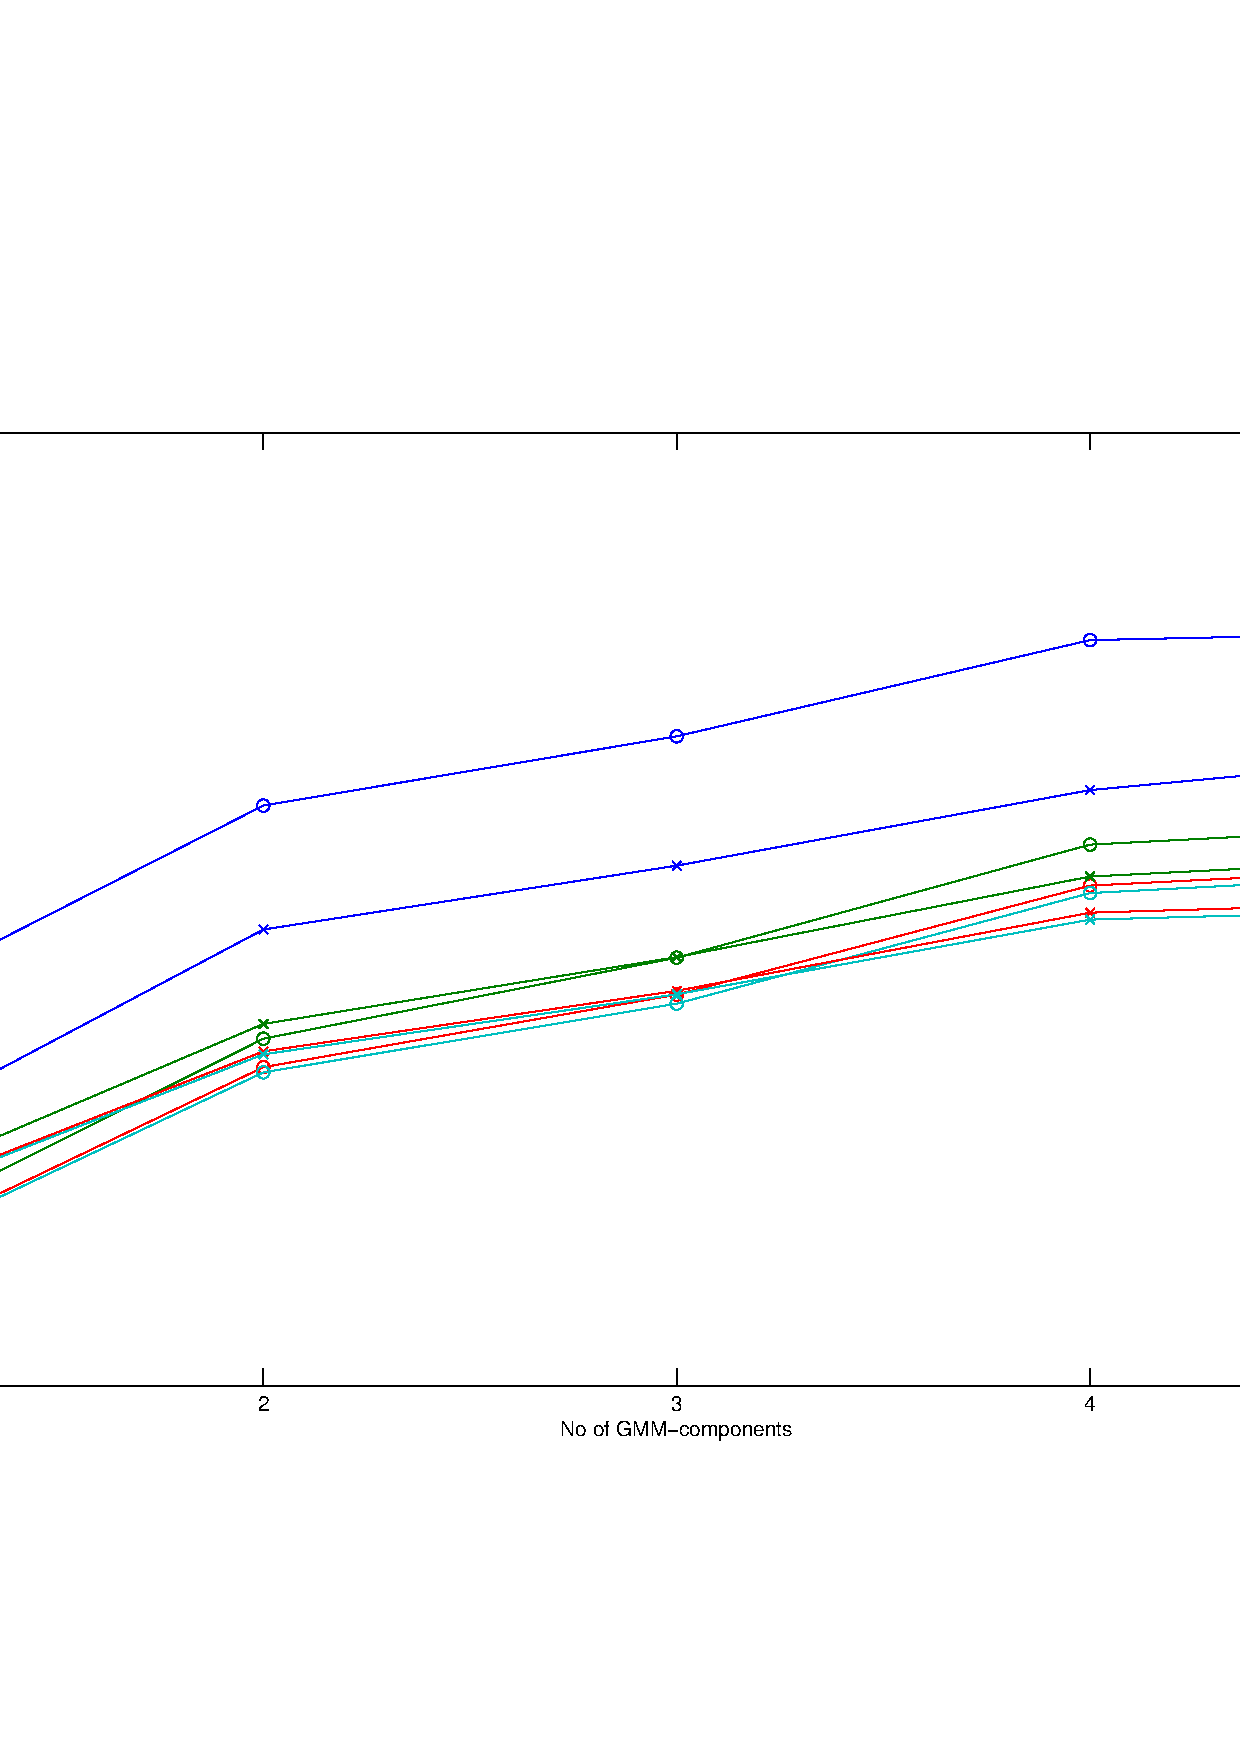
\includegraphics[width=.9\textwidth]{loss_vs.pdf}
    \caption{The average error (loss) of the classifiers on different amounts of training data, given different levels of smoothness of the data. \label{fig:loss}}
\end{figure}

Furthermore, the loss depends on the smoothness of the data: the more GMM components used per class, the higher the loss. The results show crudely the same trend as does the amount of noise with increased smoothness, so it might be the case that the increased loss is caused mainly by an increased amount of noise. Therefore, the bias and variance components of the loss were estimated separately. these results can be seen in Figures~\ref{fig:bias} and \ref{fig:var}. From Figure~\ref{fig:bias}, it is clear that the bias increases sharply when the smoothness of the data is reduced. There is little difference in the amounts of data used here, and again KNN seems to have more bias than NB on smooth data and less bias on less regular data. The variance component of the error does also increase with less smooth data, but less sharply than the bias does. Here, it becomes clear that the fact that training on small amounts of data performs less can be attributed to the higher variance, because the noise and bias don't differ significantly over this variable. It is clear too that KNN on low amounts of data is better due to a smaller variance component in the loss. For the other amounts of training data, NB seems to have consistently a little less variance.

\begin{figure}[htb]
    \centering
    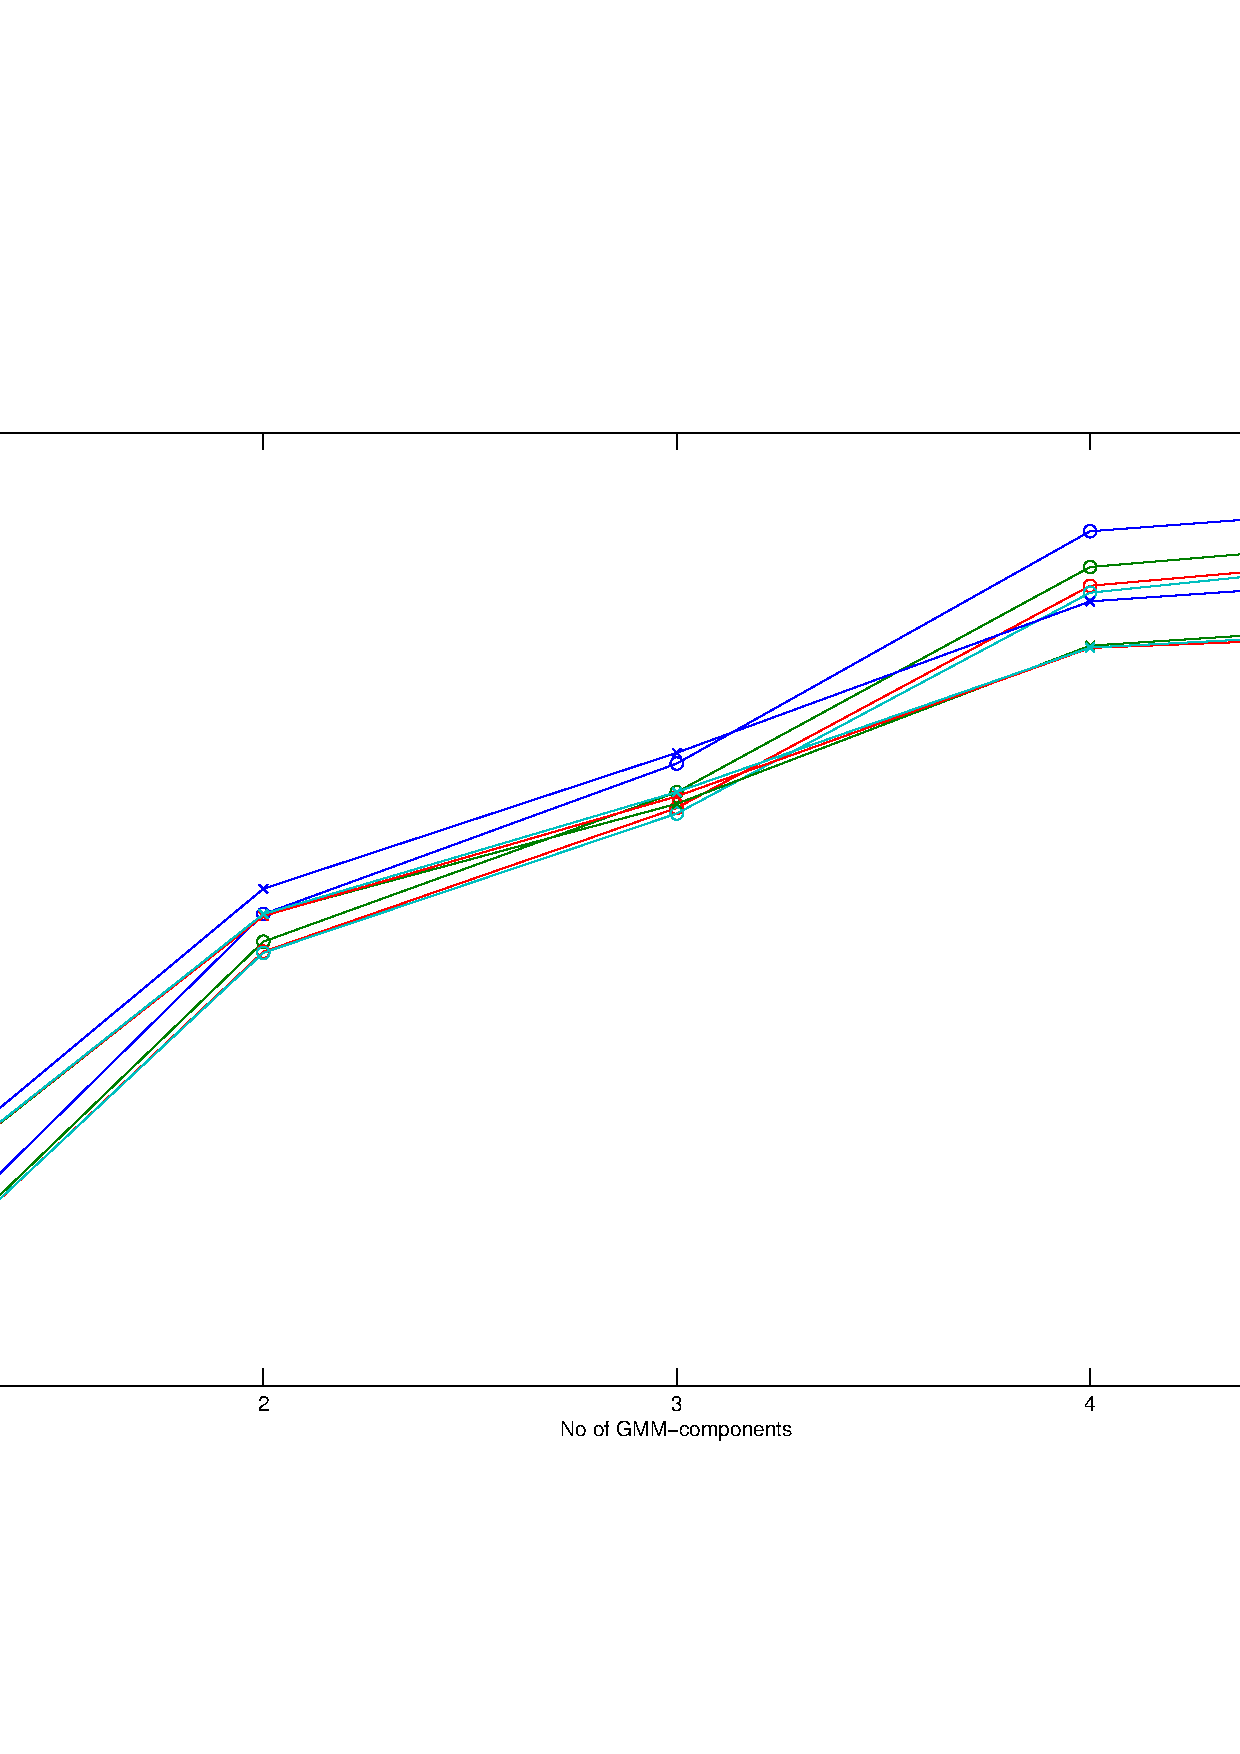
\includegraphics[width=.9\textwidth]{bias_vs.pdf}
    \caption{The average bias of the classifiers on different amounts of training data, given different levels of smoothness of the data. \label{fig:bias}}
\end{figure}

\begin{figure}[htb]
    \centering
    \includegraphics[width=.9\textwidth]{var_vs.pdf}
    \caption{The average variance of the classifiers on different amounts of training data, given different levels of smoothness of the data. \label{fig:var}}
\end{figure}

We were interested in the relation between the loss of the classifiers and the components bias, variance and noise. As was reported in several papers (\emph{cf.} \cite{Domingos2000}), this relationship can be of a complex nature, although it is generally assumed to be a sum. To find a hint about this relationship in the algorithms used, we compared the loss with the naive way of combining the components: summing. The results are shown in Figures~\ref{fig:knnlosscomp} and \ref{fig:nblosscomp}.

\begin{figure}[htb]
    \centering
    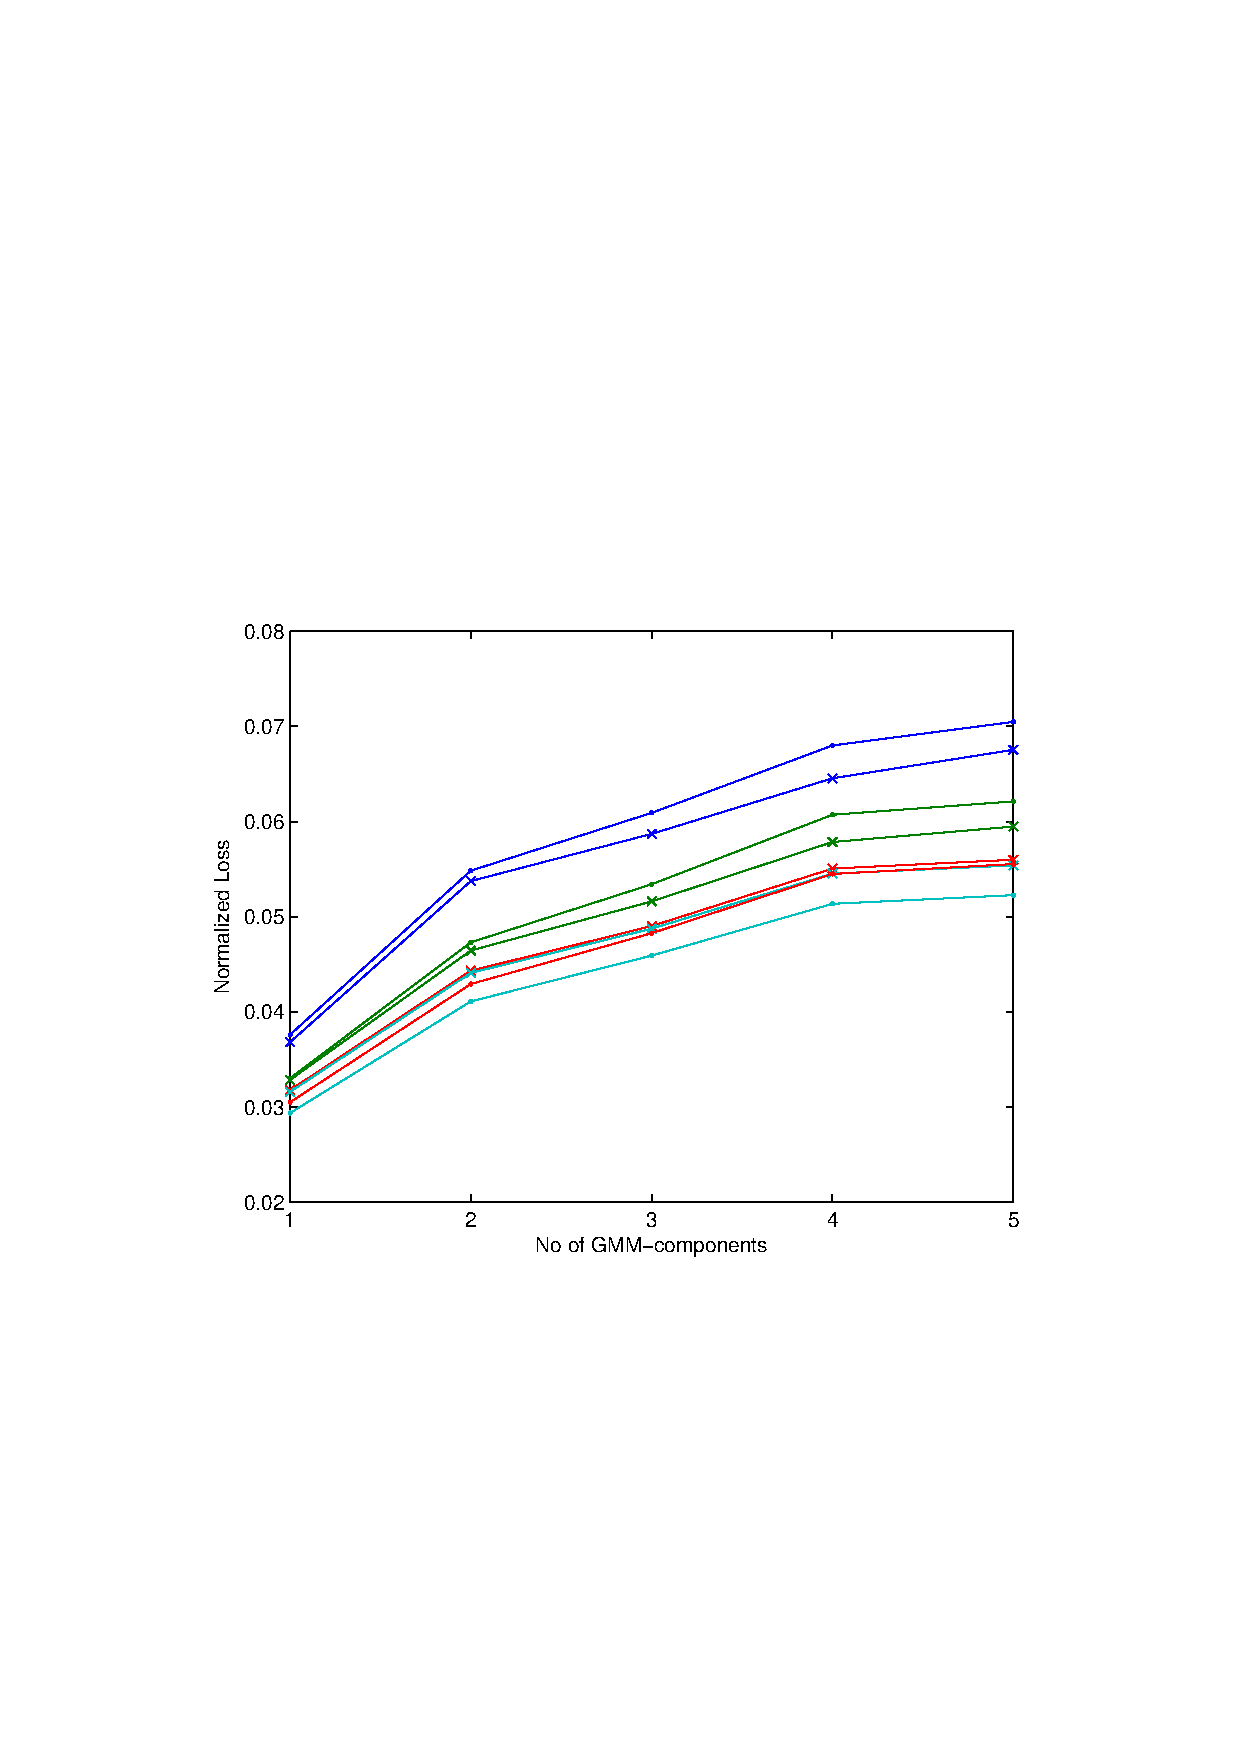
\includegraphics[width=.9\textwidth]{5040_knn_losscomp.pdf}
    \caption{KNN. Comparison of the average loss with the sum of the average bias, variance and noise. Each is normalized so all values for a data series sum to 1. \label{fig:knnlosscomp}}
\end{figure}

\begin{figure}[htb]
    \centering
    \includegraphics[width=.9\textwidth]{5050_nb_losscomp.pdf}
    \caption{Naive Bayes. Comparison of the average loss with the sum of the average bias, variance and noise. Each is normalized so all values for a data series sum to 1. \label{fig:nblosscomp}}
\end{figure}

The results show that when normalized, the loss of each classification setting is very similar to the sum of its components, which suggests a linear relationship between them. It is not a simple sum because the sum of the components tends to be larger than the loss, but the graphs suggest there is no real intricate relationship with the settings used and the classifiers used.

\section{Conclusion}



%Design choices:
% 2 class problem (2 PDFs) or concept learning problem (1 PDF versus rest). How to define the PDF (MVD, GMM, uniform)?
% Things to vary and try out: number of dimensions, real noise (next to the inherent noise), different number of components per class or number of datapoints per class, forms of PDF, learning algorithm (NB, KNN, ANN, Dec. Trees, SVM).

%Initial experiments:
% 2d 2 class
% GMM 1-5 mixtures (k) per class
% for each k:
%  m = |D| := 5 - 50 - 500 - 5000 (per class)
%  z = |T| := 1000 (500 per class)
% 100 runs each to estimate bias/variance/noise
% ?? runs each to average over different 2 class problems (e.g. pick new GMM each time)

%Workflow:
% 1. create pdfs: pick pi, mu, Sigma for each class {0,1} and k = 1-5
% 2. sample 100 datasets for each choice of k (= 400 total)
% 3. sample T
% 4. compute y_*
% 5. compute y_m = mode(t-y_*)
% 6. train classifier on each d \in D
% 7. evaluate on T
% Repeat enough times to get stable average over possible problems

%Measures:
% Accuracy: |TP|+|TN|/z
% Average bias E_x[L(y_*, y_m)]
% Average var E_x E_D[ L(y_m, y) ]
% Dataset noise L(t,y_*)

\end{document}
